% Plantilla de informe/memoria UC3M + ISCIII. Demo de titulo con
% asignatura/grupo/profesor, secciones y subsecciones, lista, tabla, figura,
% formula y enlaces.
%
% Compilar:  make      (latexmk -lualatex, dos pasadas por \pageref{LastPage})
%
% No hace falta cargar inputenc ni fontenc: bajo LuaLaTeX+fontspec la
% codificacion la gestiona el motor, y anadirlos aqui solo generaria avisos.
\documentclass[11pt,twoside]{article}

% babel va ANTES que uc3misciidoc: el paquete carga hyperref internamente, y
% hyperref necesita que babel este ya activo para traducir al espanol los
% nombres que genera \autoref (si no, salen en ingles pese a compilar en
% espanol).
\usepackage[spanish,es-noquoting]{babel}
\usepackage{uc3misciidoc}

\title{Análisis de rendimiento de un sistema distribuido de colas}
\subject{Sistemas Distribuidos}
\degree{Grado en Ingeniería Informática}
\group{Grupo 81}
\professor{Pedro Pedro Pedro}
\author{Raúl Aguilar Arroyo \and Raúl Aguilar Arroyo}
\date{Curso 2026/2027 -- Primer cuatrimestre}
\shorttitle{Rendimiento de colas distribuidas}

\begin{document}
\maketitle

\section{Introducción}

Este documento recoge el análisis de rendimiento de un sistema de colas
distribuido bajo distintos niveles de carga, realizado como memoria de la
asignatura indicada en la cabecera del título.

\subsection{Objetivos}

Se busca caracterizar la latencia y el rendimiento del sistema en función
del número de productores y consumidores activos, así como identificar el
punto a partir del cual la tasa de error deja de ser despreciable.

\subsection{Estructura del documento}

La \autoref{sec:metodologia} describe el diseño experimental; la
\autoref{sec:resultados} presenta los resultados obtenidos; la
\autoref{sec:conclusiones} resume las conclusiones.

\section{Metodología}
\label{sec:metodologia}

\subsection{Diseño experimental}

Se ha desplegado un clúster de tres nodos sobre los que se ejecuta el
sistema de colas, generando carga sintética con distintos perfiles de
llegada de peticiones.

\subsubsection{Parámetros de simulación}

Los parámetros considerados en cada configuración fueron:

\begin{itemize}
  \item Número de productores concurrentes.
  \item Número de consumidores concurrentes.
  \item Tamaño máximo de la cola.
  \item Política de reintento ante saturación.
\end{itemize}

\section{Resultados}
\label{sec:resultados}

La \autoref{tab:resultados} resume los tiempos medios de respuesta y el
rendimiento observado en cada configuración evaluada.

\begin{table}[h]
  \centering
  \caption{Tiempos medios de respuesta por configuración.}
  \label{tab:resultados}
  \begin{tabular}{@{}lrrr@{}}
    \toprule
    Configuración & Latencia (ms) & Throughput (req/s) & Error (\%) \\
    \midrule
    Baja carga    & 12  & 480  & 0,0 \\
    Carga media   & 34  & 1120 & 0,2 \\
    Carga alta    & 97  & 1780 & 1,8 \\
    Saturación    & 310 & 1825 & 9,4 \\
    \bottomrule
  \end{tabular}
\end{table}

La \autoref{fig:latencia} muestra la evolución del tiempo de respuesta a
medida que aumenta la carga sobre el sistema.

\begin{figure}[h]
  \centering
  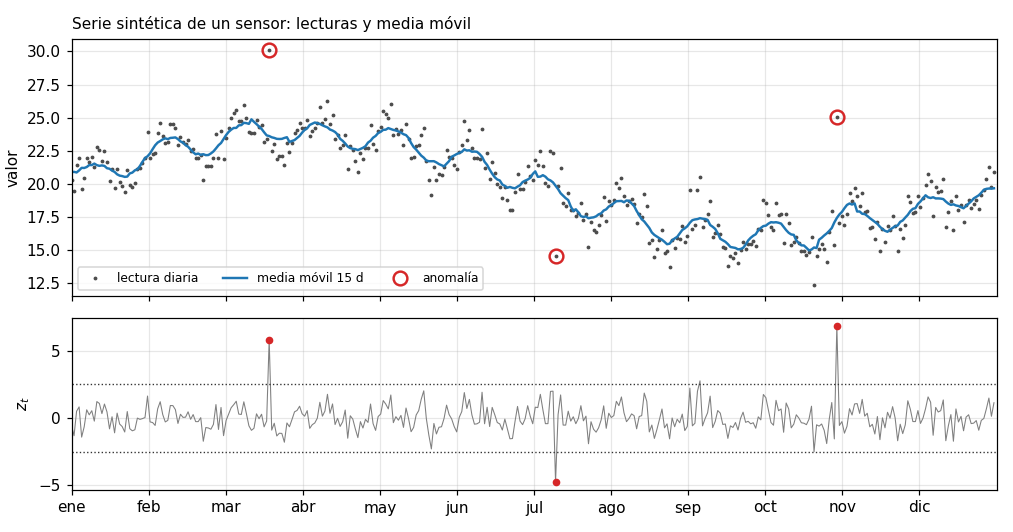
\includegraphics[width=0.7\linewidth]{figs/demo-figura}
  \caption{Evolución del tiempo de respuesta bajo carga creciente.}
  \label{fig:latencia}
\end{figure}

El tiempo medio de espera en un sistema M/M/1 viene dado por
\[
  W = \frac{\rho}{\mu - \lambda},
\]
donde $\lambda$ es la tasa de llegada, $\mu$ la tasa de servicio y
$\rho = \lambda / \mu$ la utilización del sistema~\cite{kleinrock1975}.

Los datos se han obtenido con la herramienta Locust~\cite{locust} sobre el
clúster descrito en \autoref{sec:metodologia}.

\section{Discusión}
\label{sec:discusion}

Los resultados obtenidos son consistentes con lo esperado para un sistema
de colas M/M/1: la latencia crece de forma acusada a medida que la
utilización del sistema se aproxima a uno, mientras que el throughput se
estabiliza mucho antes de llegar a ese límite. Este comportamiento es
además el esperado en un sistema distribuido con comunicación por colas
entre nodos~\cite{tanenbaum2007}.

\subsection{Limitaciones del estudio}

El experimento se ha ejecutado sobre un único perfil de llegada de
peticiones (Poisson homogéneo). Un perfil de llegada más realista, con
ráfagas de tráfico, probablemente adelantaría el punto de saturación
observado en la \autoref{sec:resultados}.

Tampoco se ha evaluado el efecto de fallos parciales del clúster (caída de
uno de los tres nodos), que podría degradar el rendimiento de forma más
brusca que un simple aumento de carga.

\subsection{Trabajo futuro}

Como continuación natural de este trabajo, se plantea repetir el
experimento con un generador de carga que incluya ráfagas, y añadir un
escenario de fallo de nodo para caracterizar la degradación del servicio
en condiciones más cercanas a un entorno de producción real.

\section{Conclusiones}
\label{sec:conclusiones}

El sistema mantiene una tasa de error despreciable hasta la configuración
de carga alta; a partir de ahí, el tiempo de respuesta crece de forma no
lineal y la tasa de error deja de ser aceptable, lo que sitúa el límite
práctico de operación justo por debajo del régimen de saturación.

\bibliographystyle{plain}
\bibliography{referencias}

\end{document}
